\chapter{軌道上最小Knudsen数地点での流体場解析結果}
\label{chap:min-knud}

希薄流の解析にはDSMC法が広く用いられるが,連続流をDSMC法で解くと大量の計算リソースと膨大な計算時間がかかるため,連続流にはNavier–Stokes解析を用いるのが一般的である.
流星源は地上に落下する以前にアブレーションによって消滅し,流星源が運動するのは高度50~km以上であるため,希薄流が支配的である可能性が高い.
従って軌道上の多くの範囲でDSMC法を使用すればよいということになる.
しかし,流星源が地上に近づいてくると大気の希薄度は下がり,連続流になる可能性も考えられる.

そこで本章では,
Navier–Stokes解析とDSMC法の使い分けが必要となるかを調査することを目的として,
流星源が人工衛星より放出されてからアブレーションによって消滅する間で,最もKnudsen数が小さくなる地点での流体場解析結果について議論する.

\section{計算条件}
\subsection{主流条件}
最小Knudsen数となった地点の主流条件を表~\ref{tab:min-knud-condition}に示す.表に示すとおり流星源直径は初期の10~mmから3.60~mmにアブレーションによって減少しており,
また最小Knudsen数ですらほとんど1に近く,遷移流であることが示されている.
\begin{table}[H]
    \centering
    \caption{最小Knudsen数地点における主流条件}
    \begin{tabular}{ll}
    \hline\hline
        流星源高度 & 73.2~km \\
        主流速度 & 6,880.0~m/s \\
        主流温度 & 219.0~K \\
        主流密度 & $3.018\times10^{-5}\ \mathrm{kg/m^3}$ \\
        流星源直径 & 3.60~mm \\
        Reynolds数 & 52.0 \\
        Knudsen数 & 0.9926 \\
    \hline\hline
    \end{tabular}
    \label{tab:min-knud-condition}
\end{table}

\subsection{Navier–Stokes解析の計算条件}
Navier–Stokes解析に用いる計算格子を図~\ref{fig:grid-ns}に示す.
半径10~cmの半円と半径1.80~mmの流星源を境界としており,流星源表面では滑りなし境界としている.
また,$x$軸上においては軸対称計算を可能にするために反射境界としている.

格子点数は$301\times301$で中心から半径方向外側に向けて指数関数的に粗くなる格子を採用した.
粘性流では壁面近傍の最小格子幅$\Delta x_{\min}$は物体表面上の境界層を捉えるために,
以下の式で与えられる格子幅程度にすればよいことが知られている~\cite{kurohon}.
\begin{equation}
    \Delta x_{\min} = L_\mathrm{ref}\dfrac{0.1}{\sqrt{Re}}
\end{equation}
ここで,$L_\mathrm{ref}$は代表長さ,$Re$はReynolds数である.
本研究では最小格子幅を\SI{2}{\micro\metre}とした.

\begin{figure}[H]
    \centering
    \includegraphics[width=10cm]{fig/min_knud/grid_ns.pdf}
    \caption{Navier–Stokes解析に用いる計算格子.}
    \label{fig:grid-ns}
\end{figure}

また,Navier–Stokes解析の他の条件としては,Courant数を0.2,壁面温度$T_\mathrm{w}$を1,000~Kとし,等温壁とした.

% \begin{table}[H]
%     \centering
%     \caption{Navier–Stokes解析における計算条件.}
%     \begin{tabular}{ll}
%     \hline\hline
%         Courant数 & 0.2 \\
%         壁面温度 & 3,000~K \\
%     \hline\hline
%     \end{tabular}
%     \label{tab:ns-setup}
% \end{table}

\subsection{DSMC法の計算条件}
DSMC法に用いる計算格子を図~\ref{fig:grid-dsmc}に示す.
計算領域は$x$方向に2~cm, $y$方向に1~cmの長方形となっている.
この長方形を$500\times250$の格子点に分割し,一辺が\SI{40}{\micro\metre}の直交等間隔格子を計算格子として採用した.

また,本研究で使用するSPARTA~\cite{spartaWWW}コードにおける固体表面は,格子を配置した後に埋め込まれ,半径1.80~mmの半円を計算領域の原点と円の中心が重なるようにして流星源を配置した.

\begin{figure}[H]
    \vspace{15mm}
    \centering
    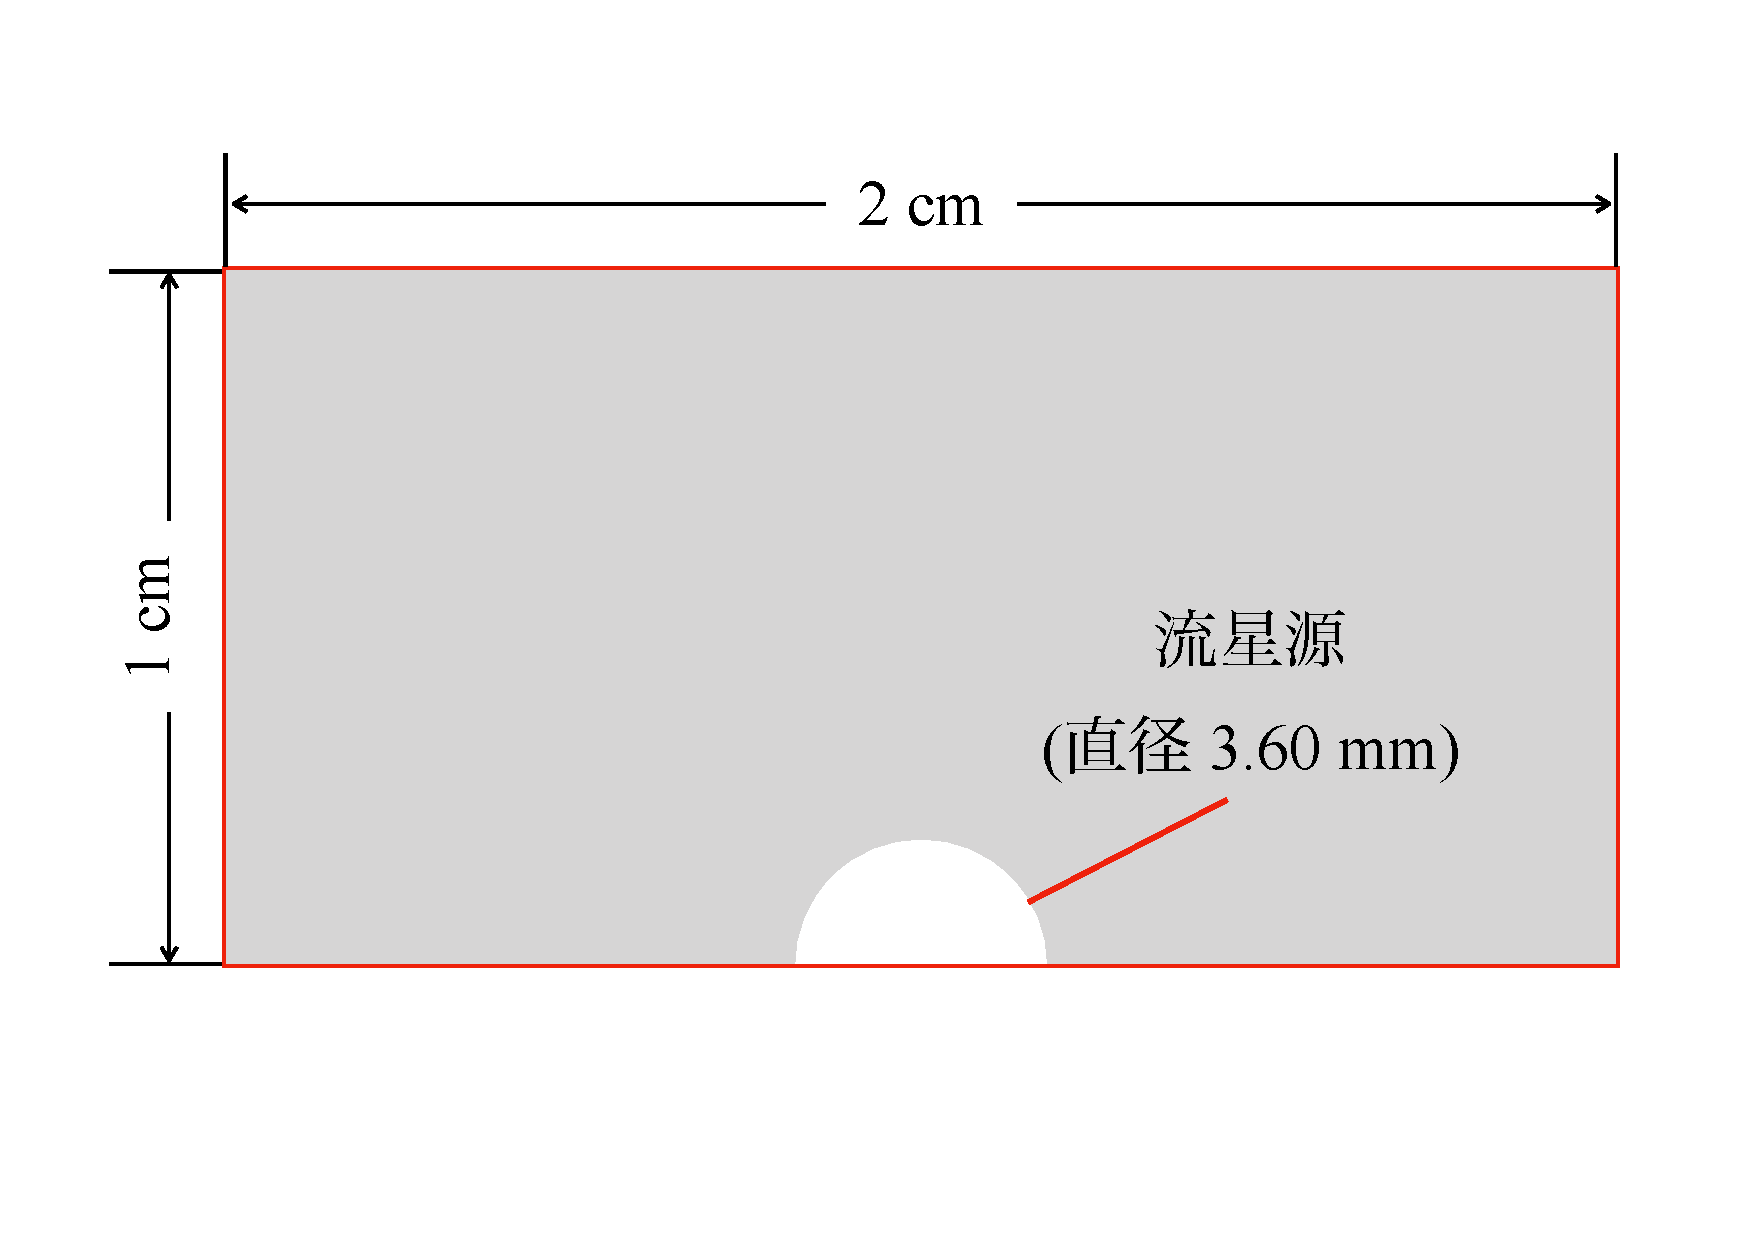
\includegraphics[width=10cm]{fig/min_knud/grid_dsmc.pdf}
    \vspace{-15mm}
    \caption{DSMC法に用いる計算格子.}
    \label{fig:grid-dsmc}
\end{figure}

また,DSMC法におけるその他の計算条件については表~\ref{tab:dsmc-setup}に示す.

\begin{table}[H]
    \centering
    \caption{DSMC法における計算条件}
    \begin{tabular}{ll}
        \hline\hline
        時間刻み幅 & \SI{1e-9}{s} \\
        衝突モデル & VSSモデル \\
        壁面反射 & 散乱反射 (適応係数1) \\
        \hline\hline
    \end{tabular}
    \label{tab:dsmc-setup}
\end{table}

\newpage
\section{流体場解析結果}
\subsection{解析結果の妥当性の検証}

%\begin{figure}[H]
%    \centering
%    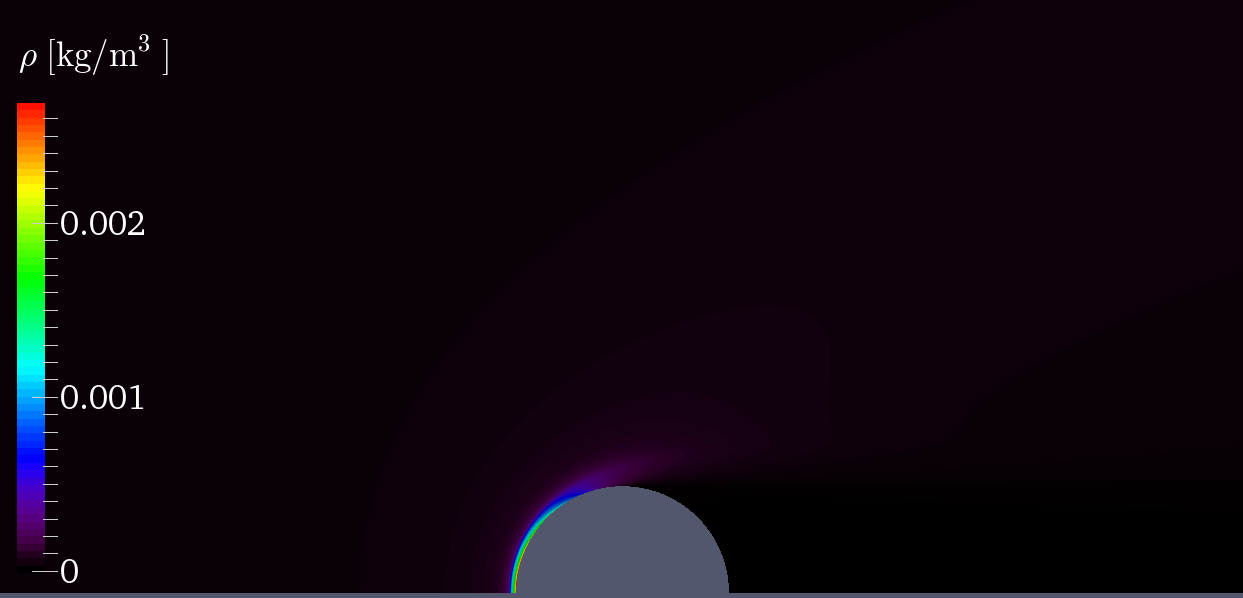
\includegraphics[width=10cm]{fig/min_knud/ns/rho.png}
%    \caption{Navier–Stokes解析での密度分布.}
%    \label{fig:ns-rho}
%\end{figure}
%\begin{figure}[H]
%    \centering
%    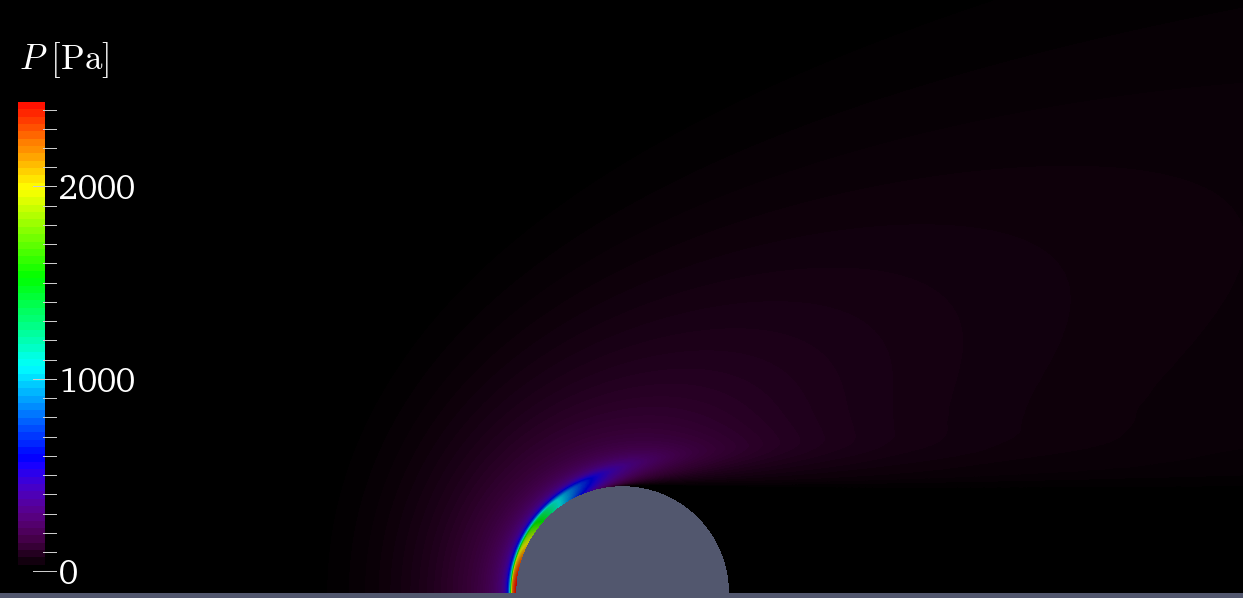
\includegraphics[width=10cm]{fig/min_knud/ns/p.png}
%    \caption{Navier–Stokes解析での圧力分布.}
%    \label{fig:ns-p}
%\end{figure}
%\begin{figure}[H]
%    \centering
%    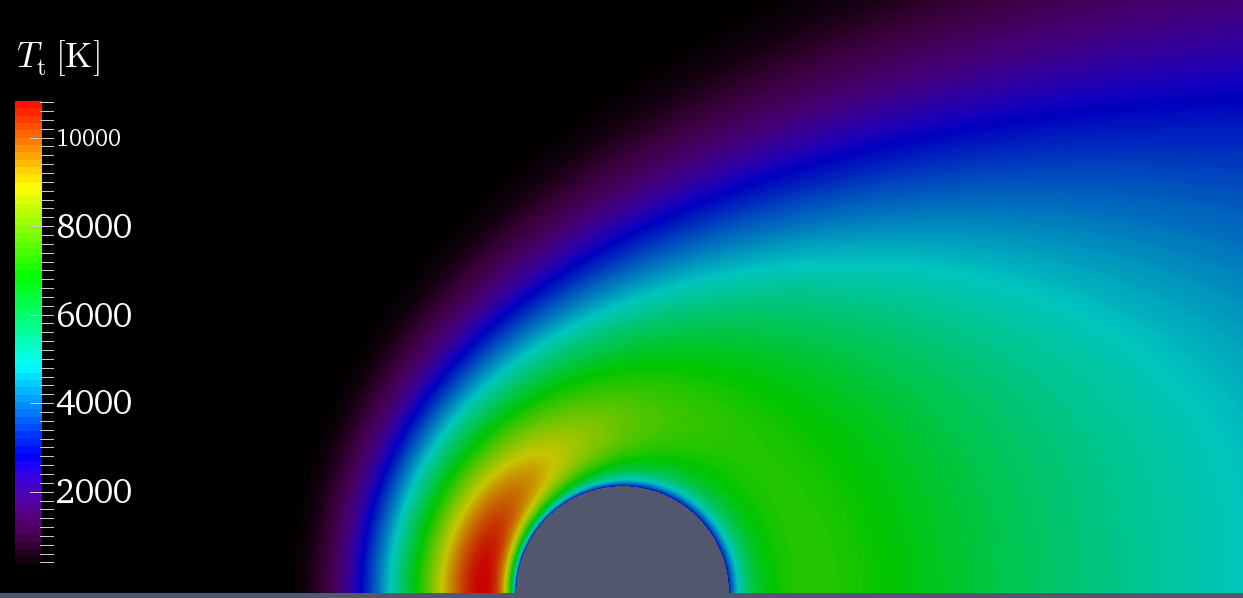
\includegraphics[width=10cm]{fig/min_knud/ns/tt.png}
%    \caption{Navier–Stokes解析での並進・回転温度分布.}
%    \label{fig:ns-tt}
%\end{figure}
%\begin{figure}[H]
%    \centering
%    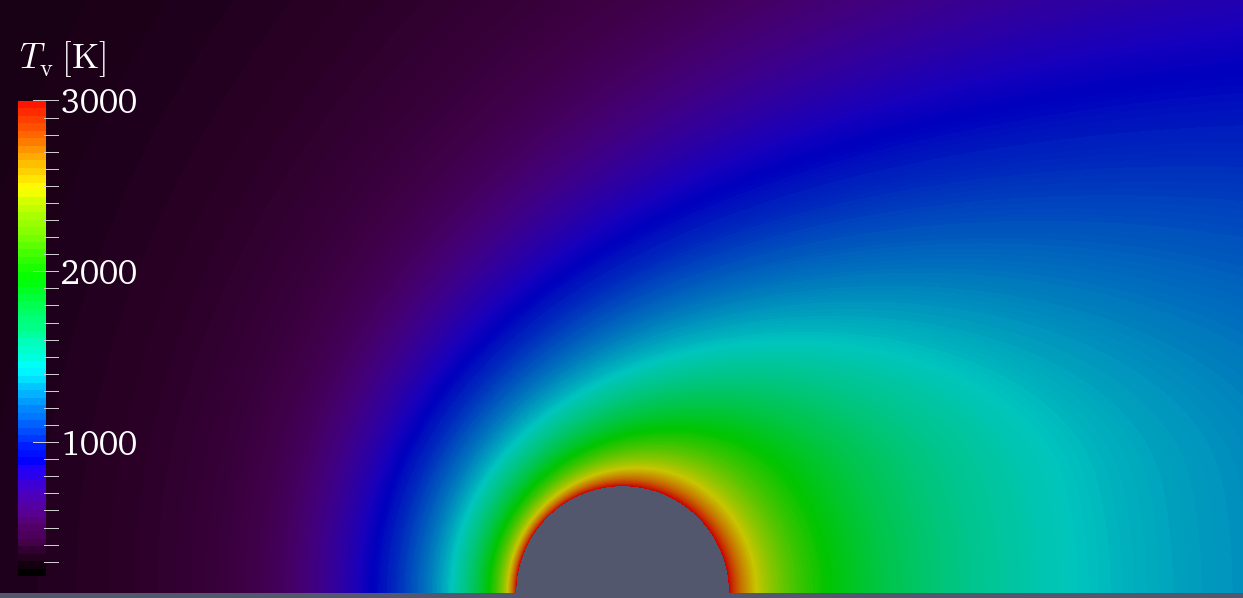
\includegraphics[width=10cm]{fig/min_knud/ns/tv.png}
%    \caption{Navier–Stokes解析での振動・励起温度分布.}
%    \label{fig:ns-tv}
%\end{figure}
%\begin{figure}[H]
%    \centering
%    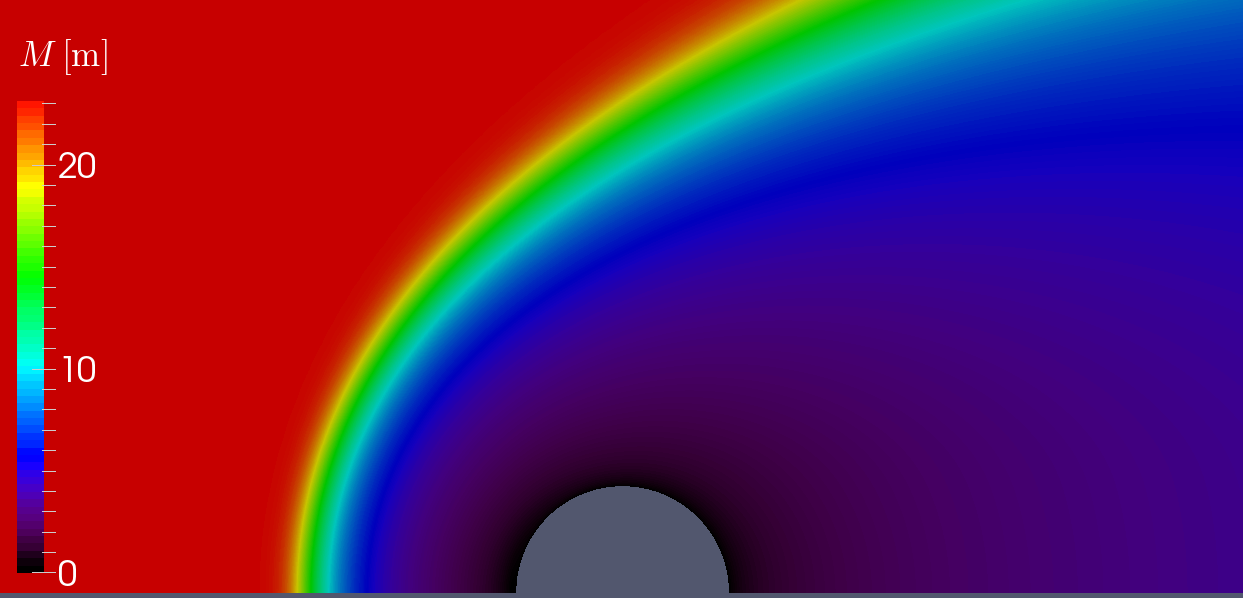
\includegraphics[width=10cm]{fig/min_knud/ns/mach.png}
%    \caption{Navier–Stokes解析でのMach数分布.}
%    \label{fig:ns-mach}
%\end{figure}
%\begin{figure}[H]
%    \centering
%    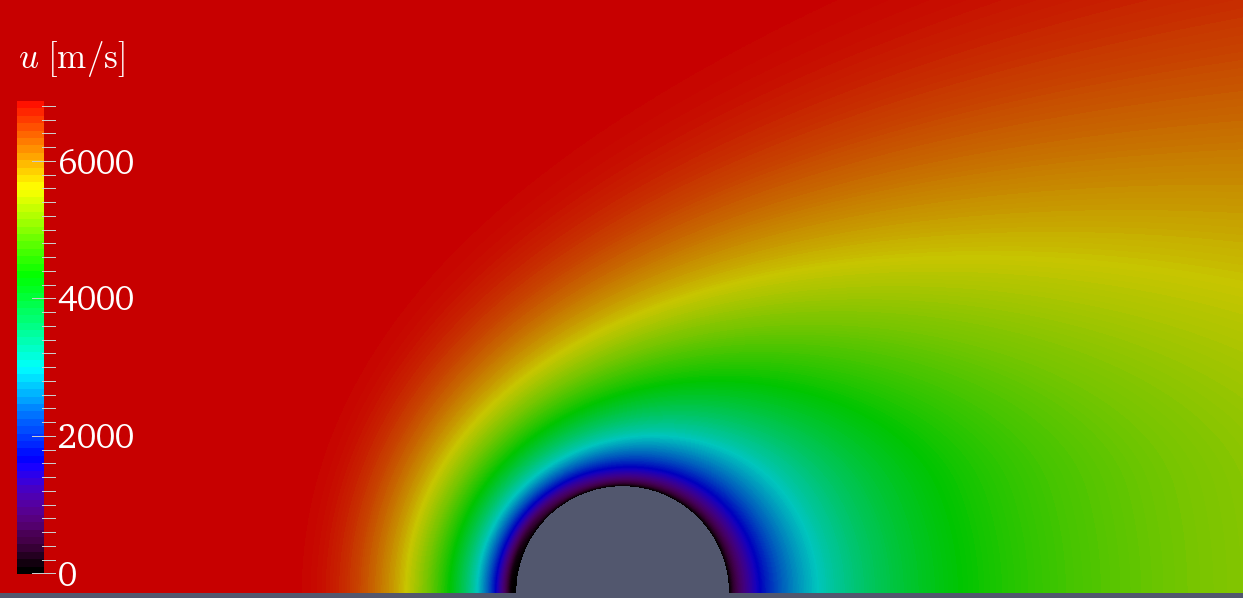
\includegraphics[width=10cm]{fig/min_knud/ns/u.png}
%    \caption{Navier–Stokes解析での$x$方向速度分布.}
%    \label{fig:ns-u}
%\end{figure}
%\begin{figure}[H]
%    \centering
%    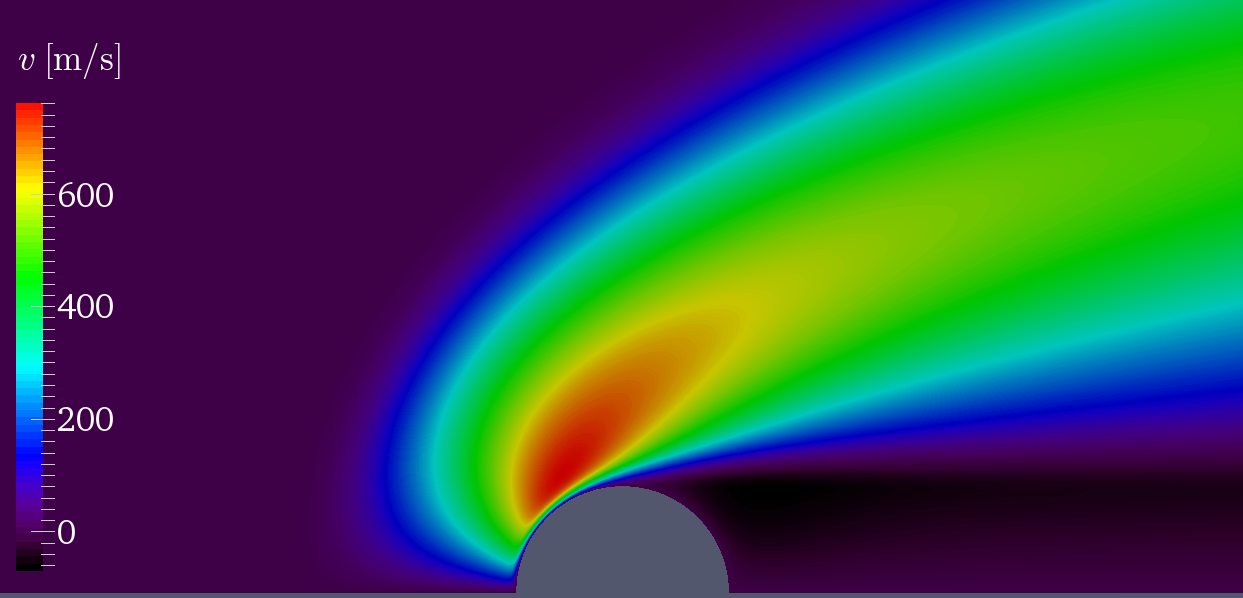
\includegraphics[width=10cm]{fig/min_knud/ns/v.png}
%    \caption{Navier–Stokes解析での$y$方向速度分布.}
%    \label{fig:ns-v}
%\end{figure}
Navier–Stokes解析での平均自由行程分布を図~\ref{fig:ns-lambda}に示す.
この図におけるカラースケールは対数でプロットしている.
ただし,平均自由行程は粘性係数より算出しており,平均速度はそのセルにおける速度の大きさとした.
平均自由行程は圧縮され密度が高くなる流星源前方で\SI{1e-4}{m}程度まで小さくなっている.
一方で,剥離による膨張領域となる流星源後流では,平均自由行程が\SI{1e-1}{m}程度まで長くなっている.
\begin{figure}[H]
    \centering
    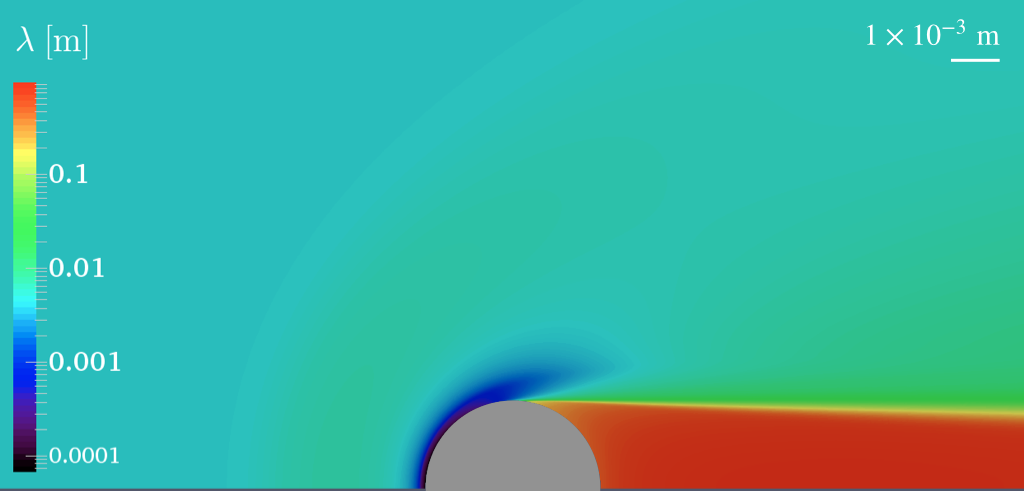
\includegraphics[width=10cm]{fig/min_knud/ns/mean_free_path.png}
    \caption{Navier–Stokes解析での平均自由行程分布.}
    \label{fig:ns-lambda}
\end{figure}

また,Navier–Stokes解析での局所Knudsen数分布を図~\ref{fig:ns-kn}に示す.
ただし,局所Knudsen数はGradient–length Local Knudsen 数$Kn_\mathrm{GLL}$~\cite{boyd1995predicting}であり,
そのセルおける平均自由行程と,物理量の勾配によるスケール長の比で算出している.
領域のほとんどでKnudsen数は1を超えており,連続体近似の破綻が示唆されている.
特に衝撃層・流星源後流において$10^2$から$10^3$程度までKnudsen数が増大している.
\begin{figure}[H]
    \centering
    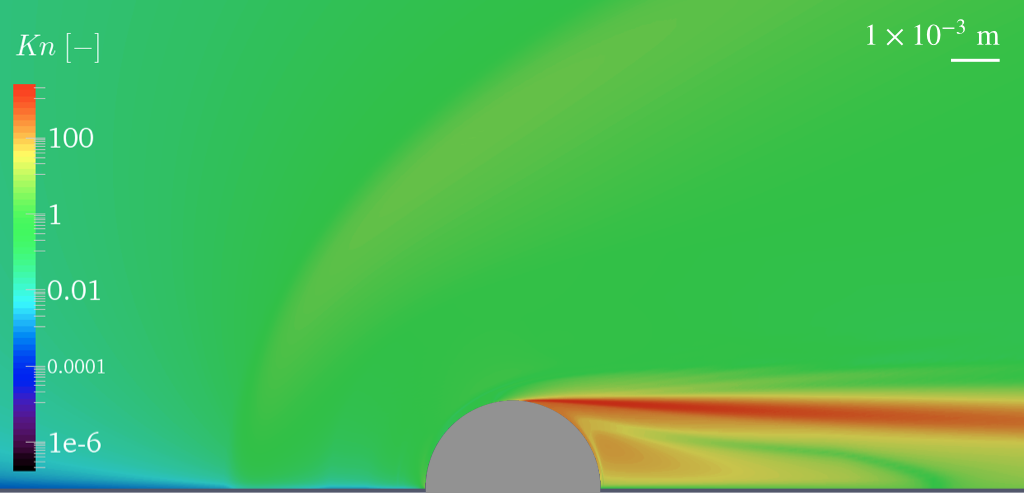
\includegraphics[width=10cm]{fig/min_knud/ns/kn.png}
    \caption{Navier–Stokes解析でのKnudsen数分布.}
    \label{fig:ns-kn}
\end{figure}
従って,最小Knudsen数高度においても局所的にもNavier–Stokes解析が適用できる領域が存在せず,
希薄流になっていることが確認された.
この結果より,流星源周りの流体場解析ではどの高度においてもDSMC法を用いればよいと考えられる.


次に,DSMC法でのサンプル粒子数を図~\ref{fig:dsmc-particle}に示す.
主流領域においては1格子あたり150以上のサンプル粒子が存在しており,
統計的に十分な数が存在している.
流星源前方では3,000を超えるサンプル粒子が存在している一方で,
流星源の後流ではサンプル粒子が回り込むことができず,
サンプル粒子が1つも存在しない領域が計算領域右端まで存在していることが分かる.
\begin{figure}[H]
    \centering
    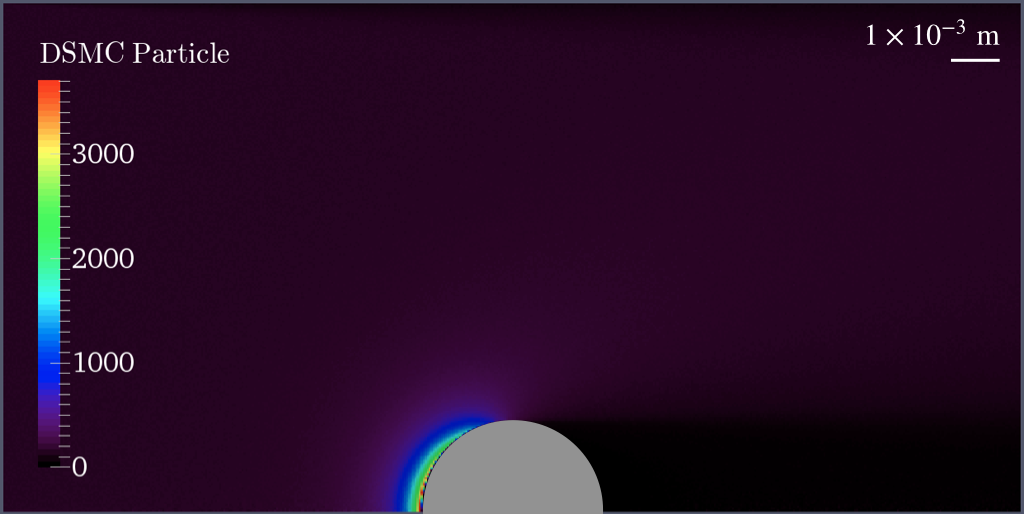
\includegraphics[width=10cm,clip]{fig/min_knud/dsmc/dsmc_particle.png}
    \caption{DSMC法でのサンプル粒子数分布.}
    \label{fig:dsmc-particle}
\end{figure}

また,DSMC法によって得られた平均自由行程とセルサイズの比の分布を示す.
ほとんどの領域で$\lambda/\Delta x$は10を超えており,平均自由行程よりも
十分小さい格子幅を取っていることが分かる.
\begin{figure}[H]
    \centering
    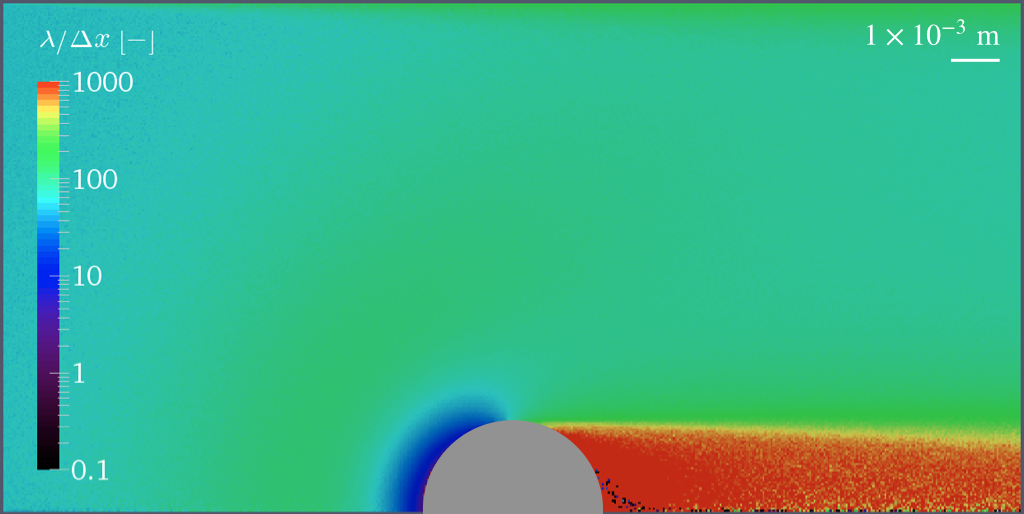
\includegraphics[width=10cm,clip]{fig/min_knud/dsmc/lambda_dx.png}
    \caption{DSMC法によって得られた平均自由行程とセルサイズの比($\lambda/\Delta x$)の分布.}
    \label{fig:dsmc-kn}
\end{figure}

ここまでの結果から,
Navier–Stokes解析は連続体近似の破綻により解析結果の信頼性が低く,
一方で本研究におけるDSMC法による解析は,
統計的に十分な粒子数や格子幅を取っていることが分かった.
以降はNavier–Stokes解析およびDSMC法で得られた巨視的な量を比較し,
どのような違いが現れるかを示す.


\subsection{速度および温度分布の比較}
Navier–Stokes解析およびDSMC法によって得られた$x$方向速度分布を図~\ref{fig:comparison-u}に示す.
流星源前方では,減速領域がDSMC法の方が厚くなっていることが分かる.
また,流星源後流においては全く異なる分布を示している.DSMC法では流星源直後から尾を引くように減速領域が存在するのに対して,
Navier–Stokes解析では楕円形に分布している.
DSMC法での結果を見ると,多次元的な広がりはほとんど無く,少しでも流星源よりも上にある主流についてはそのまま流れ去る様子が確認できる.
\begin{figure}[H]
    \centering
    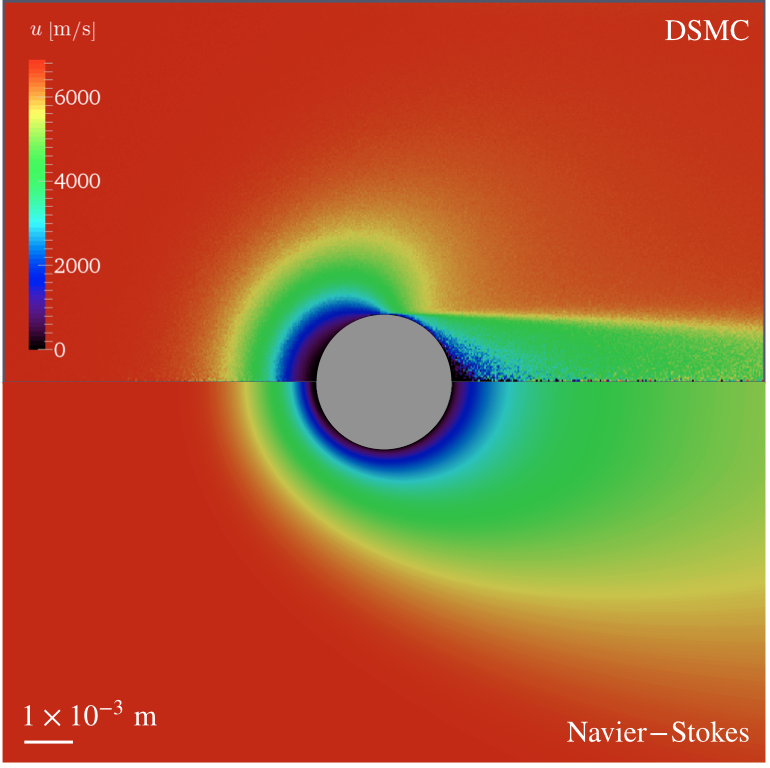
\includegraphics[width=10cm,clip]{fig/min_knud/comparison/u-crop}
    \caption{Navier–Stokes解析およびDSMC法によって得られた$x$方向速度分布.}
    \label{fig:comparison-u}
\end{figure}

また,Navier–Stokes解析およびDSMC法によって得られた$y$方向速度分布を図~\ref{fig:comparison-v}に示す.
$x$方向速度分布では大きく分布が異なったのと比較して,こちらは一致する領域が広い.
流星源前方で流星源に衝突した気体は斜め上方向へ流れていくことが分かる.
一方で,流星源直後の分布は両者で異なる.
DSMC法では$y$方向速度が負の領域が存在するが,Navier–Stokes解析ではほとんど確認できない.
この結果から,DSMC法では気体分子が後流で流星源に回り込む様子を捉えているが,
Navier–Stokes解析では見られないことが分かる.
\begin{figure}[H]
    \centering
    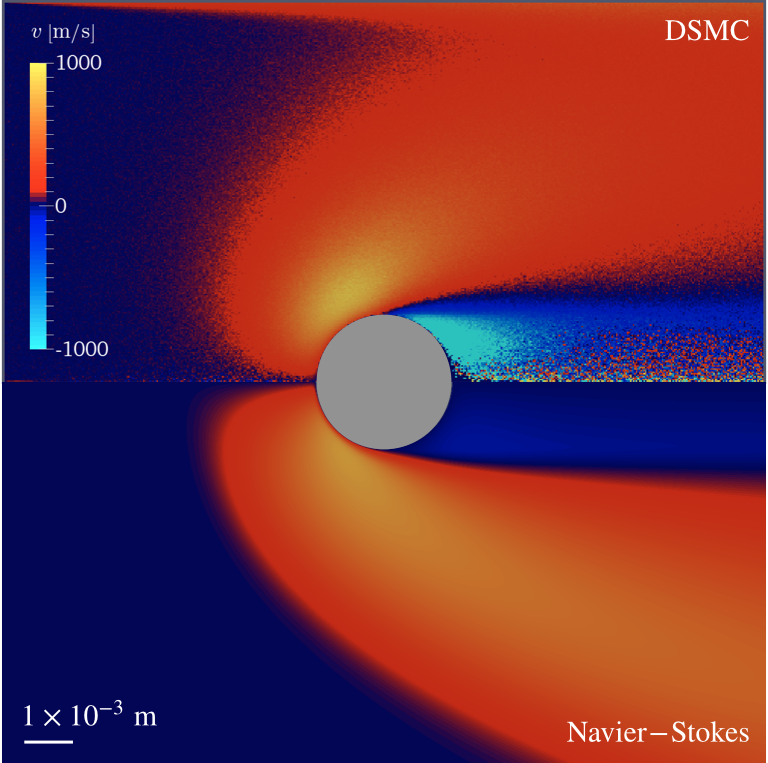
\includegraphics[width=10cm,clip]{fig/min_knud/comparison/v-crop.png}
    \caption{Navier–Stokes解析およびDSMC法によって得られた$y$方向速度分布.}
    \label{fig:comparison-v}
\end{figure}

また,Navier–Stokes解析およびDSMC法によって得られた並進温度分布を図~\ref{fig:comparison-tt}に示す.
淀み点は,DSMC法で約18,800~K,Navier–Stokes解析で約10,800~Kであり,DSMC法において約1.6倍ほど大きく見積もられた.
さらに,流星源前方の衝撃層の厚みも異なっており,DSMC法の方が厚くなっている.
衝撃層の厚さは,平均自由行程程度になることが知られており~\cite{maruzen圧縮性流体},
流星源直径と同程度の平均自由行程である本主流条件では,
DSMC法においてその特性をよく表すことができている.
さらに,$x$方向速度分布と似た後流形状をしていることから,流星源表面で気体分子が滑るか否かが
大きく後流に影響していると考えられる.
\begin{figure}[H]
    \centering
    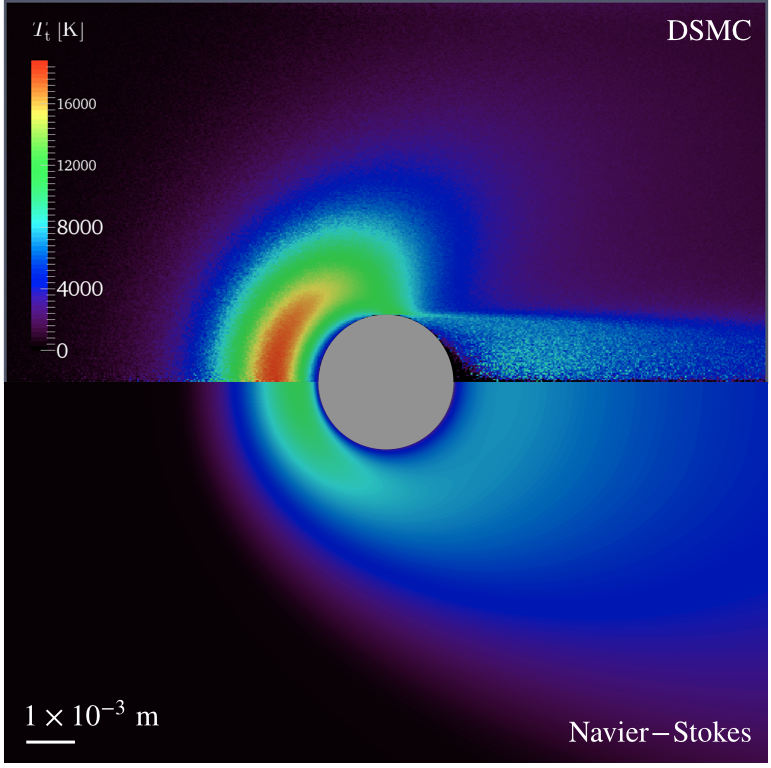
\includegraphics[width=10cm,clip]{fig/min_knud/comparison/tt-crop}
    \caption{Navier–Stokes解析およびDSMC法によって得られた並進温度分布.}
    \label{fig:comparison-tt}
\end{figure}

また,DSMC法で得られた分布において,計算領域の上境界で勾配が確認される.
上境界の境界条件は流出境界としており,この境界から出ていくサンプル粒子は単純に消去される.
図~\ref{fig:comparison-v}を見ると明らかなように,この境界では上方向に速度を持っていることがわかる.
計算領域左端での流入境界から入ってきた粒子は$y$方向速度を持たないが,
上境界で値を与えていないためにDSMC法の結果に勾配が現れたと考えられる.
この勾配の大きさは衝撃層での勾配と比べて無視できるほど小さいとこに加え,
流星源から離れた位置に形成されるため影響は無視できると考えられる.

\newpage
\section{淀み点熱流束による比較}
淀み点を0度とし,流星源表面位置を方位角で表したときの熱流束分布を図~\ref{fig:min-knud-heat-flux}に示す.
ここで,黒い鎖線で示すのは軌道計算に用いたDKRモデルによって見積もられた淀み点熱流束である.

また,軌道計算において対流熱流束の推算に用いているDKRモデルによる熱流束と,
Navier–Stokes解析およびDSMC法によって得られた淀み点における熱流束の比較を表~\ref{tab:heat-flux}に示す.
軌道計算に用いたDKRモデルで見積もられた熱流束である約\SI{8}{MW/m^2}を基準として比較すると,DKRモデルでの熱流束に対してNavier–Stokes解析は約9割に過小評価された.
一方DKRモデルでの熱流束に対するDSMC法での熱流束は,約5割と大きく過小評価されたことが分かる.

本計算条件の全体Knudsen数はほとんど1に達し,Navier–Stokes解析から局所的にも連続流領域がほとんど存在しておらず,希薄流になっている可能性が極めて高い.
仮にDSMC法により見積もられた淀み点熱流束がNavier–Stokes解析の見積もりよりも実際の物理現象をより良く再現できていると仮定すれば,
この結果から軌道計算における熱流束の予測には希薄流にも対応したDKRモデル以外のモデルを使用するか,
DKRモデルで得られる熱流束を何らかの方法で補正する必要があると考えられる.

\begin{figure}[H]
    \centering
    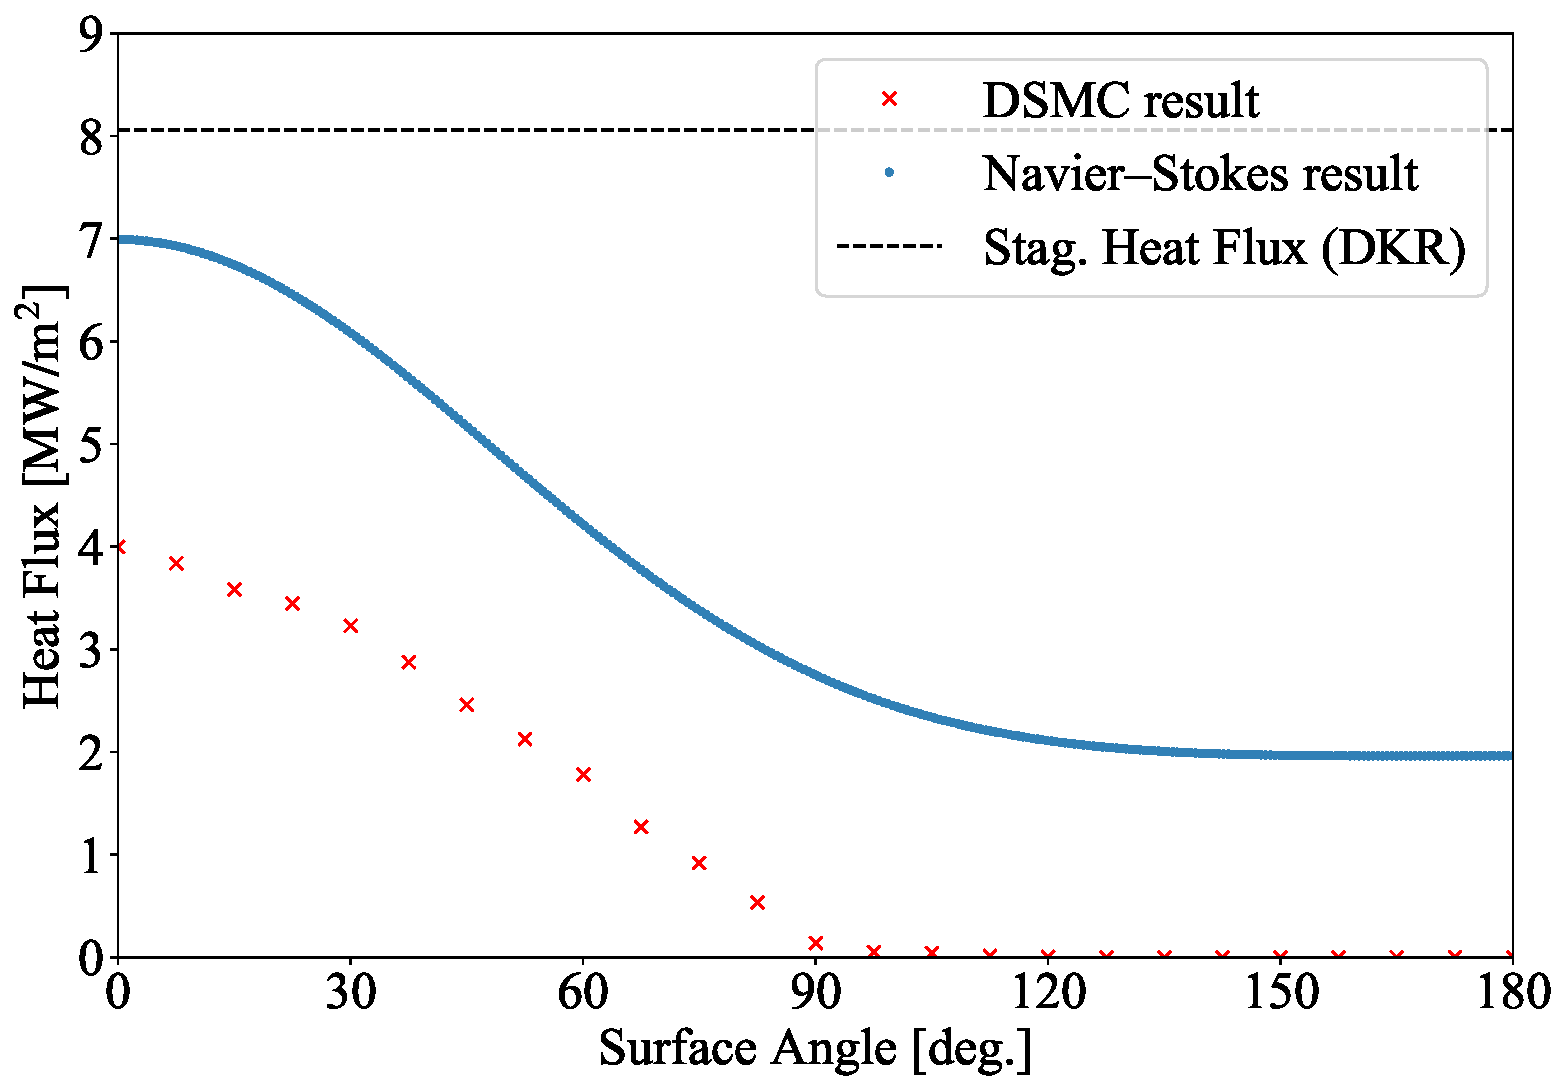
\includegraphics[width=10cm]{fig/min_knud/heat-flux-magni.pdf}
    \caption{DKRモデルによる淀み点熱流束と流星源表面における熱流束.}
    \label{fig:min-knud-heat-flux}
\end{figure}

\begin{table}[H]
    \centering
    \caption{淀み点における熱流束の比較.}
    \begin{tabular}{c|ccc}
        \hline\hline
         & DKRモデル & Navier–Stokes解析 & DSMC法 \\ \hline
        淀み点熱流束~[\si{MW/m^2}] & 8.057 & 6.994 & 3.998 \\
        DKR モデルとの比~[–] & – & 0.87 & 0.49 \\
        \hline\hline
    \end{tabular}
    \label{tab:heat-flux}
\end{table}

Navier–Stokes解析とDSMC法による流れ場解析では大きく異なる結果を得た.
Knudsen数を考慮すると連続体近似は破綻しており,DSMC法が適している考えられるが,
本研究での流体場解析結果を用いた明確な根拠を示すことができなかったため,
今後実験値や理論値~\cite{singh2016heat,singh2017aerothermodynamic}との比較を行い,
DSMC法が人工流れ星周りの流体場解析に適していることを示す必要がある.

%\section{本章のまとめ}
%本章では,軌道上において最小Knudsen数をとる高度73~kmにおける,
%Navier–Stokes解析及びDSMC法による流体場解析を行った.
%主流のKnudsen数がほとんど1であることに加えて,
%Navier–Stokes解析によって得られた局所Knudsen数もほとんどの領域で1を超え,特に後流では$10^2$以上のKnudsen数になった.
%また,DSMC法におけるサンプル粒子数や格子幅は統計的に適正な範囲であり,
%従ってNavier–Stokes解析よりもDSMC法が適していることが示唆された.
%
%2つの解析手法によって得られた速度分布・温度分布を見ると,
%流星源前方で一致する領域があるものの,特に後流場において全く異なる分布を示した.
%温度分布において,淀み点温度はDSMC法が約1.6倍に大きく見積もられ,
%後流のみならず前方においても流体場の特性が異なることが分かった.
%
%Navier–Stokes解析と比較してDSMC法が本条件に適している可能性は極めて高いが,
%DSMC法がより適している決定的な根拠を示すことができなかった.
%そのため今後は理論解や実験値との比較を行う必要があると言える.
%
%また,淀み点における熱流束を軌道計算に用いたDKRモデルと比較した.
%Navier–Stokes解析での淀み点熱流束はDKRモデルの87\%,DSMC法では49\%に見積もられ,
%連続流を仮定しているDKRモデルはDSMC法で得られる結果と異なることが分かった.
%仮にDSMC法が実際の物理現象に近いとすると,
%この淀み点熱流束違いはアブレーションに影響し,
%軌道計算の熱流束の見積もりに対する修正が求められることが分かった.